\documentclass[conference]{IEEEtran}
\IEEEoverridecommandlockouts
\usepackage{cite}
\usepackage{amsmath,amssymb,amsfonts}
\usepackage{graphicx}
\usepackage{textcomp}
\usepackage{xcolor}
\usepackage{booktabs}
\usepackage{url}

\def\BibTeX{{\rm B\kern-.05em{\sc i\kern-.025em b}\kern-.08em
    T\kern-.1667em\lower.7ex\hbox{E}\kern-.125emX}}

\begin{document}

\title{Detecci\'on de Residuos Reciclables en una Cinta Transportadora con YOLOv8: una Comparaci\'on de Pol\'iticas de Aumentaci\'on}

\author{
\IEEEauthorblockN{Julia Maldonado, Alejandro Valle, Mar\'ia Gabriela Di Grazia, Byron Garc\'ia}
\IEEEauthorblockA{
Carrera de Especializaci\'on en Inteligencia Artificial (CEIA)\\
Facultad de Ingenier\'ia, Universidad de Buenos Aires (FIUBA)\\
Visi\'on por Computadora II --- Grupo 6
}
}

\maketitle

\begin{abstract}
Los centros de acopio reciben residuos mezclados cuya separaci\'on manual es lenta y costosa.
Este trabajo propone un sistema de visi\'on por computadora que, instalado sobre una cinta
transportadora, detecta y clasifica residuos en seis categor\'ias (biodegradable, cart\'on,
vidrio, metal, papel y pl\'astico) para priorizar la extracci\'on de los materiales de mayor
valor de reciclaje. Se entrenaron y compararon cuatro configuraciones -- dos variantes de
YOLOv8 (n y s) bajo dos pol\'iticas de aumentaci\'on de datos -- sobre un conjunto de 10.464
im\'agenes (dataset Garbage Classification 3, Roboflow). La pol\'itica de aumentaci\'on
propuesta, dise\~nada a partir de un an\'alisis cuantitativo de las carencias del dataset
(orientaci\'on, iluminaci\'on y nitidez), mejor\'o el mAP@0.5:0.95 en +1,2 puntos (YOLOv8s) y
+0,7 puntos (YOLOv8n) frente a la configuraci\'on por defecto de Ultralytics, con YOLOv8s +
proposed alcanzando 0,650 de mAP@0.5 y 55 FPS en una GPU T4.
\end{abstract}

\begin{IEEEkeywords}
detecci\'on de objetos, YOLOv8, clasificaci\'on de residuos, aumentaci\'on de datos, visi\'on
por computadora, reciclaje.
\end{IEEEkeywords}

\section{Introducci\'on}

En ciudades concurridas se genera una gran cantidad de basura mezclada. Separarla
manualmente, material por material, es lento y costoso, y gran parte del material reciclable
pierde valor comercial por no identificarse y extraerse a tiempo durante el procesamiento.
Clasificar directamente en la v\'ia p\'ublica, durante la recolecci\'on, es poco pr\'actico por
las condiciones de iluminaci\'on y movimiento; resulta m\'as viable automatizar la
clasificaci\'on una vez que el residuo llega a un centro de acopio o planta de procesamiento,
donde puede pasar por una cinta transportadora bajo condiciones controladas de c\'amara.

El objetivo de este trabajo es dise\~nar y evaluar un sistema de detecci\'on de objetos basado
en deep learning que, sobre una cinta transportadora, identifique en tiempo real la categor\'ia
de cada residuo y permita priorizar la extracci\'on de los materiales de mayor valor de
reciclaje (por ejemplo, aluminio, PET o cart\'on), en lugar de requerir una separaci\'on
exhaustiva del 100\% del flujo. El alcance de este trabajo se concentra en el problema de
visi\'on por computadora --- detecci\'on y clasificaci\'on de los distintos tipos de residuos
--- dejando la implementaci\'on f\'isica del mecanismo de separaci\'on (brazo mec\'anico o aire
a presi\'on) como una extensi\'on futura de la aplicaci\'on.

Como antecedente de un caso real, Koskinopoulou et al.~\cite{koskinopoulou2021} describen un
sistema de categorizaci\'on basado en visi\'on por computadora para la separaci\'on rob\'otica
industrial de residuos reciclables, desplegado y evaluado en una planta de procesamiento de
residuos real, bajo condiciones industriales exigentes, utilizando un m\'odulo de visi\'on de
bajo costo basado en deep learning. En la industria, Recycleye reporta un caso de despliegue en
la planta de materiales recuperables (MRF) de re3 en Reading, Reino Unido, con 99\% de pureza
del material separado frente a 96\% en la l\'inea de separaci\'on humana de referencia y hasta
55 extracciones por minuto~\cite{recycleye2022}. Ambos antecedentes respaldan la viabilidad de
un enfoque de visi\'on por computadora para esta tarea, aunque las cifras de la industria no
est\'an auditadas de forma independiente, a diferencia de las m\'etricas reportadas en este
trabajo.

\section{Metodolog\'ia}

\subsection{Conjunto de datos y procesamiento}

Se utiliz\'o el dataset p\'ublico Garbage Classification 3 (v2, formato YOLOv8) de
Roboflow~\cite{roboflow2024}, con 10.464 im\'agenes anotadas en seis clases: biodegradable,
cardboard, glass, metal, paper y plastic. Previo al entrenamiento se audit\'o el export crudo
para descartar im\'agenes corruptas y corregir o eliminar anotaciones defectuosas --- un paso
necesario porque los exports de Roboflow pueden contener errores de etiquetado que de otro
modo perjudican el entrenamiento de forma silenciosa. Se re-dividi\'o el dataset en una
partici\'on propia 70/20/10 (train/val/test) en lugar de conservar la de Roboflow, que
resultaba desbalanceada entre clases y habr\'ia invalidado la evaluaci\'on por clase. El
conjunto de test se mantuvo reservado y sin aumentar hasta la evaluaci\'on final.

\subsection{Pol\'itica de aumentaci\'on}

Las t\'ecnicas de aumentaci\'on se eligieron a partir de un an\'alisis cuantitativo del dataset
procesado --- no de supuestos gen\'ericos --- midiendo brillo, nitidez, color y balance de
clases. El an\'alisis mostr\'o que al dataset le faltan im\'agenes oscuras o borrosas,
condiciones esperables en video real de una cinta transportadora, y que el desbalance de
clases observado se debe a la cantidad de objetos por foto y no a la cantidad de fotos por
clase. A partir de esos hallazgos se definieron dos configuraciones (\emph{arms}) para
comparar: \texttt{ultralytics\_defaults}, la aumentaci\'on por defecto de
Ultralytics~\cite{ultralytics2023} (mosaico, jitter HSV, flip horizontal, traslaci\'on y
escala), y \texttt{proposed}, que a\~nade flip vertical, oscurecimiento (reducci\'on de brillo
de hasta -40\% con probabilidad 0,3), motion blur y Gaussian blur, para cubrir las carencias
medidas de orientaci\'on, iluminaci\'on y nitidez, implementadas con
Albumentations~\cite{buslaev2020}. La aumentaci\'on se aplica en forma \emph{online} durante el
entrenamiento, a partir de un \'unico archivo de configuraci\'on compartido, de modo que todas
las corridas usan exactamente la misma pol\'itica y el conjunto de test nunca se aumenta por
accidente.

\subsection{Entrenamiento y evaluaci\'on}

Se realiz\'o fine-tuning de dos variantes pre-entrenadas de YOLOv8~\cite{ultralytics2023} ---
YOLOv8n y YOLOv8s --- bajo cada una de las dos pol\'iticas de aumentaci\'on, resultando en
cuatro configuraciones entrenadas. Cada modelo se entren\'o durante 50 \'epocas, batch size 16
y semilla fija (42), sobre una GPU T4 (Google Colab). La evaluaci\'on se realiz\'o sobre el
conjunto de test reservado, reportando mAP@0.5, mAP@0.5:0.95, F1 y latencia de inferencia
extremo a extremo (200 im\'agenes de test, procesadas una por una), medida tanto en GPU T4 como
en CPU de notebook (Intel i5-1135G7).

\section{Resultados Experimentales y An\'alisis}

La Tabla~\ref{tab:metricas} resume las m\'etricas de las cuatro configuraciones sobre el
conjunto de test. La pol\'itica \texttt{proposed} super\'o a \texttt{ultralytics\_defaults} en
ambas arquitecturas: +1,2 puntos de mAP@0.5:0.95 en YOLOv8s y +0,7 puntos en YOLOv8n. La
mejora se observ\'o en cinco de las seis clases en ambos modelos, con una \'unica excepci\'on
menor en CARDBOARD (-0,008), lo que sugiere que el oscurecimiento y el desenfoque agregados por
la pol\'itica propuesta ayudan de forma consistente sin introducir una regresi\'on relevante.

\begin{table}[htbp]
\caption{M\'etricas por modelo y receta (conjunto de test)}
\begin{center}
\begin{tabular}{llccc}
\toprule
\textbf{Modelo} & \textbf{Receta} & \textbf{mAP@0.5} & \textbf{mAP@.5:.95} & \textbf{F1} \\
\midrule
YOLOv8s & proposed             & 0.650 & 0.467 & 0.650 \\
YOLOv8s & ultralytics\_defaults & 0.645 & 0.455 & 0.646 \\
YOLOv8n & proposed             & 0.629 & 0.443 & 0.625 \\
YOLOv8n & ultralytics\_defaults & 0.622 & 0.435 & 0.617 \\
\bottomrule
\end{tabular}
\label{tab:metricas}
\end{center}
\end{table}

YOLOv8s super\'o a YOLOv8n en las seis clases bajo ambas recetas, a cambio de mayor latencia:
en GPU T4, YOLOv8s + proposed proces\'o cada imagen en 18,1~ms (55~FPS) frente a 10,2~ms
(98~FPS) de YOLOv8n + proposed. En CPU (Intel i5-1135G7, pesos \texttt{proposed}), YOLOv8n
alcanz\'o 68,9~ms (14,5~FPS) frente a 177,3~ms (5,6~FPS) de YOLOv8s --- una diferencia de 2,6$\times$
relevante para un despliegue sin GPU dedicada.

El modelo recomendado es YOLOv8s con la pol\'itica \texttt{proposed}, por tener el mejor
mAP@0.5:0.95 y F1 del conjunto y correr en tiempo real sobre GPU (55~FPS). Para un despliegue
sin GPU se recomienda YOLOv8n + \texttt{proposed} como alternativa, con una ca\'ida de 2,4
puntos de mAP@0.5:0.95 a cambio de ser 2,6$\times$ m\'as r\'apido en CPU. Las clases con peor
desempe\~no en ambos modelos son BIODEGRADABLE, CARDBOARD y PAPER (mAP@0.5:0.95 entre 0,36 y
0,43 en YOLOv8s), consistente con la variabilidad visual de esos materiales.

\subsection{Demostraci\'on sobre una cinta simulada}

Para ilustrar el funcionamiento del sistema sin una cinta f\'isica se construy\'o una
simulaci\'on: 11 im\'agenes del conjunto de test (elegidas al azar con semilla fija), cada una
reescalada a un cuadrado de 420~px, se deslizan de izquierda a derecha sobre un fondo de banda
de 1280$\times$540~px, a 30~FPS durante 20~s (600 cuadros), como si pasaran frente a una
c\'amara fija. El modelo recomendado (YOLOv8s + \texttt{proposed}, umbral de confianza 0,25) se
ejecuta cuadro por cuadro, igual que lo har\'ia un sistema en l\'inea. La
Fig.~\ref{fig:demo} muestra seis cuadros representativos.

\begin{figure*}[t]
\centering
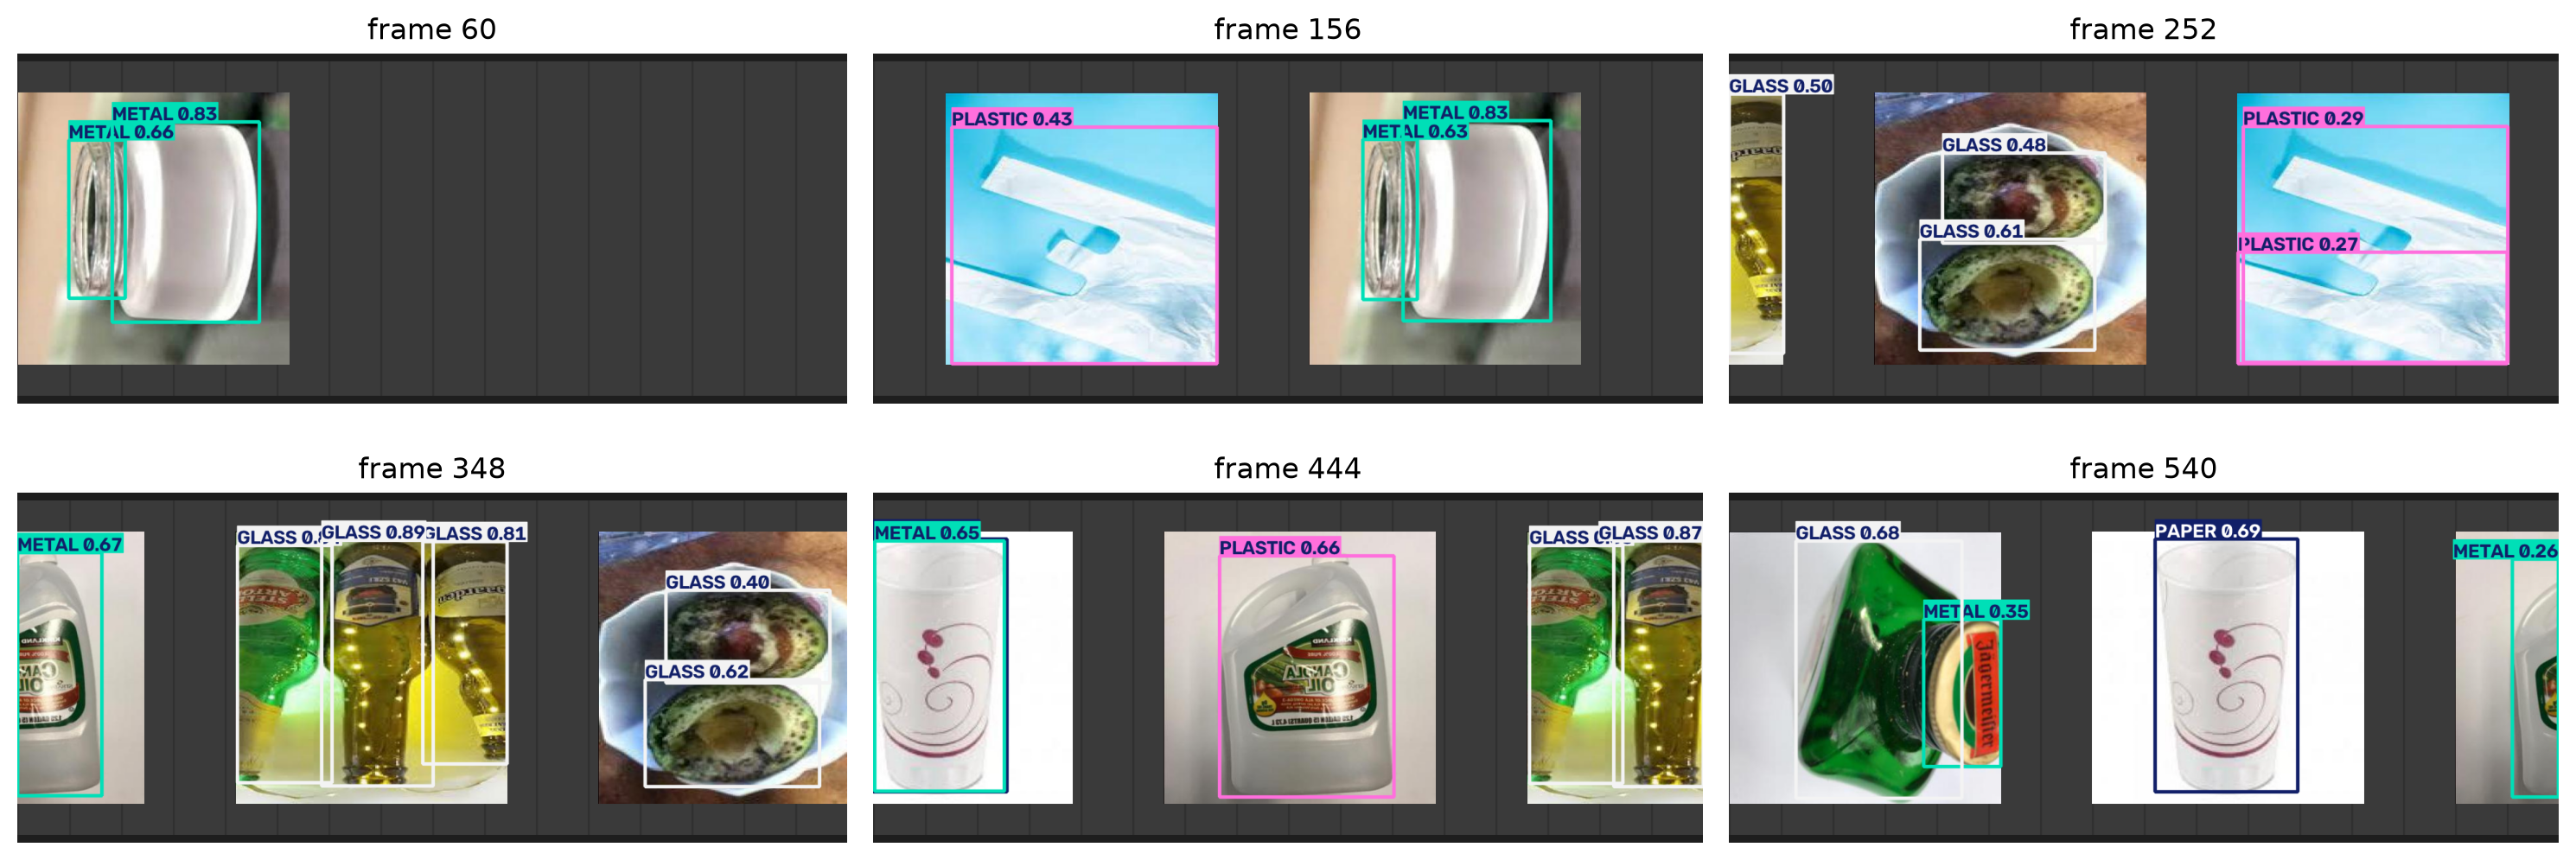
\includegraphics[width=\textwidth]{demo_frames.png}
\caption{Seis cuadros de la demostraci\'on sobre la cinta simulada, con las detecciones del
modelo YOLOv8s + \texttt{proposed}. Se observan aciertos (botellas de vidrio, vaso de papel) y
confusiones entre clases, en particular METAL.}
\label{fig:demo}
\end{figure*}

La latencia por cuadro (preprocesado, inferencia y NMS) fue de 22,9~ms en promedio (43,7~FPS) y
13,3~ms en el percentil 95, ejecutando sobre la GPU integrada (backend MPS) de un MacBook Pro.
Que el promedio supere al percentil 95 indica que unos pocos cuadros iniciales fueron mucho m\'as
lentos (calentamiento del dispositivo); en r\'egimen estable el modelo qued\'o por encima de los
30~FPS del video simulado.

\begin{table}[htbp]
\caption{Detecciones por clase en la demostraci\'on (conteo por cuadro)}
\begin{center}
\begin{tabular}{lcc}
\toprule
\textbf{Clase} & \textbf{Detecciones} & \textbf{Confianza media} \\
\midrule
GLASS         & 1241 & 0.616 \\
METAL         &  746 & 0.617 \\
PLASTIC       &  482 & 0.487 \\
PAPER         &  188 & 0.686 \\
BIODEGRADABLE &   53 & 0.554 \\
CARDBOARD     &    5 & 0.396 \\
\bottomrule
\end{tabular}
\label{tab:demo}
\end{center}
\end{table}

La Tabla~\ref{tab:demo} cuenta detecciones \emph{por cuadro}: un mismo objeto aparece en muchos
cuadros consecutivos, de modo que la tabla refleja las im\'agenes que recorrieron la banda y no
la cantidad de objetos distintos (para ello har\'ia falta seguimiento, ver Conclusiones). En los
cuadros inspeccionados se observaron dos comportamientos. Por un lado, los objetos de apariencia
clara se clasifican con confianza alta, por ejemplo las botellas de vidrio verdes (0,81 a 0,89).
Por otro, aparecen confusiones que las m\'etricas agregadas de test no hacen visibles: un mismo
bid\'on pl\'astico blanco se etiquet\'o como PLASTIC (0,66) en un cuadro y como METAL (0,67) en
otro; un vaso de papel se etiquet\'o como PAPER (0,69) y, al entrar por el borde de la banda
parcialmente recortado, como METAL (0,65); un frasco de vidrio se etiquet\'o como METAL; y los
restos de aguacate en un recipiente se etiquetaron como GLASS en lugar de BIODEGRADABLE. La
clase se vuelve inestable cuando el objeto aparece cortado en el borde del encuadre, un
escenario que el test sobre im\'agenes completas no mide. CARDBOARD casi no se detect\'o (5
detecciones, confianza media 0,396), coherente con su bajo desempe\~no en test. Estas
observaciones son cualitativas y se basan en 11 im\'agenes distintas, por lo que no sustituyen la
evaluaci\'on cuantitativa de la Tabla~\ref{tab:metricas}.

Limitaciones: cada modelo y receta se entren\'o una \'unica vez, por lo que las diferencias
reportadas no fueron sometidas a un test de significancia estad\'istica. De las cuatro recetas
definidas en la pol\'itica de aumentaci\'on, solo dos (\texttt{ultralytics\_defaults} y
\texttt{proposed}) fueron efectivamente entrenadas; \texttt{no\_augmentation} y
\texttt{proposed\_low\_saturation} quedan como trabajo futuro. Las matrices de confusi\'on se
calcularon sobre el conjunto de validaci\'on, no sobre el de test. Adem\'as, el dataset
utilizado, aunque realista, no replica completamente el nivel de desorden visual (objetos
superpuestos, oclusiones parciales) que literatura especializada documenta en video real de
cintas transportadoras~\cite{bashkirova2022}; validar el modelo recomendado contra im\'agenes
propias de la banda, m\'as cercanas a ese escenario, queda como un paso natural antes de un
despliegue productivo.

\section{Conclusiones}

\begin{enumerate}
\item Una pol\'itica de aumentaci\'on dise\~nada a partir de carencias medidas
cuantitativamente en el dataset (orientaci\'on, iluminaci\'on, nitidez) mejora el
mAP@0.5:0.95 de forma consistente frente a los valores por defecto de Ultralytics, en ambas
arquitecturas evaluadas, sin necesidad de recolectar m\'as datos.

\item YOLOv8s ofrece mejor precisi\'on que YOLOv8n en las seis clases bajo ambas recetas, pero
a un costo de latencia relevante en CPU (2,6$\times$ m\'as lento que YOLOv8n), por lo que la
elecci\'on entre ambos depende directamente del hardware de despliegue disponible en el centro
de acopio.

\item Re-dividir el dataset en lugar de usar la partici\'on original de Roboflow fue necesario
para obtener una evaluaci\'on por clase confiable, dado el desbalance detectado en la
partici\'on original.

\item Las clases BIODEGRADABLE, CARDBOARD y PAPER concentran el menor desempe\~no del sistema,
lo que sugiere que la ambig\"uedad visual entre materiales org\'anicos y de fibra es el cuello
de botella principal a resolver en una futura iteraci\'on, m\'as que la arquitectura del
detector en s\'i.

\item La demostraci\'on sobre una cinta simulada corri\'o a 43,7~FPS en una GPU integrada (MPS),
por encima de los 30~FPS del video, pero mostr\'o confusiones que el test no revela, sobre todo
METAL frente a PLASTIC, PAPER y GLASS, y clases inestables cuando el objeto queda cortado en el
borde del encuadre. Esto refuerza que el siguiente paso es validar con im\'agenes propias de la
banda y con objetos parcialmente visibles.

\item Como trabajo futuro, la arquitectura puede extenderse incorporando seguimiento de
objetos (\emph{tracking}) para evitar contar el mismo residuo dos veces en video, y evaluando
directamente la implementaci\'on f\'isica del mecanismo de separaci\'on, que qued\'o fuera del
alcance de este trabajo.
\end{enumerate}

\bibliographystyle{ieeetr}
\bibliography{references}

\end{document}
